\documentclass[../main.tex]{subfiles}

\begin{document}
\chapter{Mistakes, We've Drawn a Few}
Source: \url{https://shorturl.at/GJNQW}

\section{Truncating the Scale}
\subsection{corrected}
\begin{figure}[h]
  \centering
  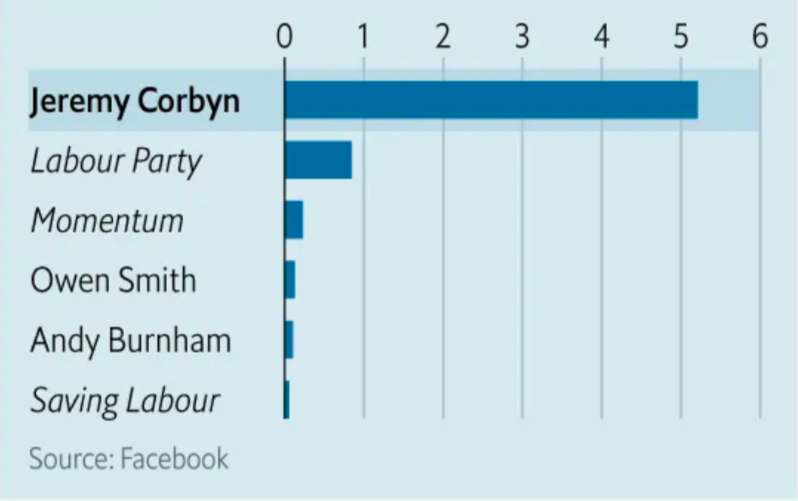
\includegraphics[width=0.6\textwidth]{
    ../graphics/correct-left-click.png
  } 
\end{figure}

\noindent
Replication.

\pgfplotstableread[%
col sep=comma,%
colums/name/.style=string type%
]{%
  ./data/corbyn/corbyn-data.csv%
}\datatable

\begin{figure}[h]
  \centering

  \begin{tikzpicture}[
    background rectangle/.style={
      fill=plotBackground
    },
    show background rectangle
    ]
    
    \begin{axis}[
      xbar,
      xmin=0,
      xticklabel pos=upper,
      enlarge x limits={value=0.2, upper},
      x coord trafo/.code={\pgfmathparse{\pgfmathresult/1000}},
      xticklabel=\pgfmathprintnumber{\tick},
      x axis line style={draw=none},
      xmajorgrids=true,
      % y axis
      yticklabels from table={\datatable}{name},
      ytick=data,
      y dir=reverse,
      axis y line=left,
      enlarge y limits=0.1,
      y axis line style={-,thick},
      % general
      tick style={draw=none},
      bar width=0.45cm,
      ]
      \addplot[plotBlue, fill=plotBlue]
      table [y expr=\coordindex, x=count] {\datatable};
   \end{axis}
   \node[below left,color=gray] () {\small Source: Facebook};
  \end{tikzpicture}
\end{figure}


\end{document}